% XCircuit output "BJT_iv.tex" for LaTeX input from BJT_iv.ps
\def\putbox#1#2#3#4{\makebox[0in][l]{\makebox[#1][l]{}\raisebox{\baselineskip}[0in][0in]{\raisebox{#2}[0in][0in]{\scalebox{#3}{#4}}}}}
\def\rightbox#1{\makebox[0in][r]{#1}}
\def\centbox#1{\makebox[0in]{#1}}
\def\topbox#1{\raisebox{-0.60\baselineskip}[0in][0in]{#1}}
\def\midbox#1{\raisebox{-0.20\baselineskip}[0in][0in]{#1}}
   \scalebox{0.8}{
   \normalsize
   \parbox{4.27604in}{
   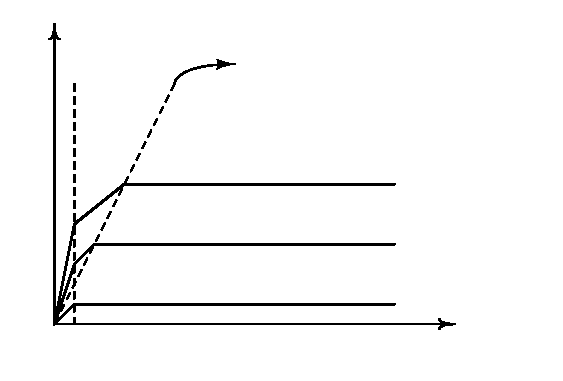
\includegraphics[scale=1.25]{BJT_iv}\\
   % translate x=287 y=291 scale 0.30
   \putbox{1.36in}{1.88in}{1.20}{aktiv. oblast}%
   \putbox{0.31in}{1.75in}{1.20}{\rotatebox{-270}{sat.}}%
   \putbox{0.56in}{1.92in}{1.20}{kvazi-}%
   \putbox{0.06in}{2.50in}{1.20}{$I_C$}%
   \putbox{3.40in}{0.09in}{1.20}{$U_{CE}$}%
   \putbox{1.90in}{2.50in}{1.20}{odpor drift.\\oblasti}%
   \putbox{0.56in}{1.75in}{1.20}{sat.}%
   } % close 'parbox'
   } % close 'scalebox'
   \vspace{-\baselineskip} % this is not necessary, but looks better
